% ****** Start of file apssamp.tex ******
%
%   This file is part of the APS files in the REVTeX 4.2 distribution.
%   Version 4.2a of REVTeX, December 2014
%
%   Copyright (c) 2014 The American Physical Society.
%
%   See the REVTeX 4 README file for restrictions and more information.
%
% TeX'ing this file requires that you have AMS-LaTeX 2.0 installed
% as well as the rest of the prerequisites for REVTeX 4.2
%
% See the REVTeX 4 README file
% It also requires running BibTeX. The commands are as follows:
%
%  1)  latex apssamp.tex
%  2)  bibtex apssamp
%  3)  latex apssamp.tex
%  4)  latex apssamp.tex
%
\documentclass[%
 reprint,
%superscriptaddress,
%groupedaddress,
%unsortedaddress,
%runinaddress,
%frontmatterverbose, 
%preprint,
%preprintnumbers,
%nofootinbib,
%nobibnotes,
%bibnotes,
 amsmath,amssymb,
 aps,
%pra,
%prb,
%rmp,
%prstab,
%prstper,
%floatfix,
]{revtex4-2}

\usepackage{graphicx}% Include figure files
\usepackage{svg}
\usepackage{tikz}
\usepackage{hyperref}
\usepackage{dcolumn}% Align table columns on decimal point
\usepackage{bm}% bold math
%\usepackage{hyperref}% add hypertext capabilities
%\usepackage[mathlines]{lineno}% Enable numbering of text and display math
%\linenumbers\relax % Commence numbering lines

%\usepackage[showframe,%Uncomment any one of the following lines to test 
%%scale=0.7, marginratio={1:1, 2:3}, ignoreall,% default settings
%%text={7in,10in},centering,
%%margin=1.5in,
%%total={6.5in,8.75in}, top=1.2in, left=0.9in, includefoot,
%%height=10in,a5paper,hmargin={3cm,0.8in},
%]{geometry}

\begin{document}

\preprint{APS/123-QED}

\title{Manuscript Title:\\with Forced Linebreak}% Force line breaks with \\
\thanks{A footnote to the article title}%

\author{Ann Author}
 \altaffiliation[Also at ]{Physics Department, XYZ University.}%Lines break automatically or can be forced with \\
\author{Second Author}%
 \email{Second.Author@institution.edu}
\affiliation{%
 Authors' institution and/or address\\
 This line break forced with \textbackslash\textbackslash
}%

\collaboration{MUSO Collaboration}%\noaffiliation

\author{Charlie Author}
 \homepage{http://www.Second.institution.edu/~Charlie.Author}
\affiliation{
 Second institution and/or address\\
 This line break forced% with \\
}%
\affiliation{
 Third institution, the second for Charlie Author
}%
\author{Delta Author}
\affiliation{%
 Authors' institution and/or address\\
 This line break forced with \textbackslash\textbackslash
}%

\collaboration{CLEO Collaboration}%\noaffiliation

\date{\today}% It is always \today, today,
             %  but any date may be explicitly specified

\begin{abstract}
An article usually includes an abstract, a concise summary of the work
covered at length in the main body of the article. 
\begin{description}
\item[Usage]
Secondary publications and information retrieval purposes.
\item[Structure]
You may use the \texttt{description} environment to structure your abstract;
use the optional argument of the \verb+\item+ command to give the category of each item. 
\end{description}
\end{abstract}

%\keywords{Suggested keywords}%Use showkeys class option if keyword
                              %display desired
\maketitle

%\tableofcontents

\section{Introduction}


\section{BDI in one dimension}

\subsection{The flow of a parity flipping, skew symmetric, unitary matrix}
Let $U$ be a unitary matrix that is quasidiagonal in one dimension, as shown in \cite{kitaev2006} we define its flow by:
\begin{equation}
    \mathcal{F}(U)=\sum_{j\le\eta<k}\left(|U_{jk}|^2-|U_{kj}|^2\right)
\end{equation}
and it can be shown that $\mathcal{F}(U)$ is an integer and independent of $\eta$. For quadratic Hamiltonians in the Majorana basis, the covariance matrix $\Gamma$, which is defined as:
\begin{equation}
    \Gamma_{jk}=\frac{i}{2}\langle[c_j,c_k]\rangle
\end{equation}
is also real and skew symmetric, therefore $\mathcal{F}(\Gamma)$ is trivially zero.
When the Hamiltonian has Time Reversal Symmetry (TRS), which acts on the Majorana ladder operators as following:
\begin{equation}
    \mathcal{T}c_{2j-1}\mathcal{T}^{-1}=-c_{2j-1}, \; \mathcal{T}c_{2j}\mathcal{T}^{-1}=c_{2j}
\end{equation}
then $\Gamma$ is forced to be parity-flipping:
\begin{equation}
    \forall i,j \; \Gamma_{2i,2j}=\Gamma_{2i-1,2j-1}=0
\end{equation}
We denote the odd-even sub matrix by $(\Gamma_{oe})_{ij}=\Gamma_{2i-1,2j}$, and not that it is unitary if $\Gamma$ is parity-flipping, and thus has a non-trivial flow $\nu(\Gamma)=\mathcal{F}(\Gamma_{oe})$. 
To calculate $\nu(\Gamma)$ using $\Gamma$ we use the partial transpose as was defined in \cite{shap2017}:
\begin{equation}
    \begin{split}
    T_{jk} &= \left\{ \begin{matrix} \delta_{jk} & j \le 0 \\ i(-1)^j\delta_{jk} & j>0 \end{matrix}\right. \\
    \tilde\Gamma &= T\Gamma T
    \end{split}
\end{equation}
There is no need to cut specifically at $0$, as long as the cut is on an even index, cutting between neighboring physical sites. \\
Using $\tilde\Gamma$ we can calculate $\nu(\Gamma)$ as following:
\begin{equation}
    \nu(\Gamma) = \frac{-Im\left(Tr(\Gamma\tilde\Gamma)\right)}{2}
\end{equation}
Since $\Gamma$ is quasidiagonal, the trace of $Im(\Gamma\tilde\Gamma)$ can be calculated only using a finite region surrounding the cut.

\subsection{Computation of $Z_\mathcal{T}$ for Free Fermions}
As was defined in \cite{shap2017}, we consider two adjacent intervals $I_{1.2}$ and compute
\begin{equation}
    Z_{\mathcal{T}}=tr(\rho_IU_{I_2}\rho_I^{T_2}U_{I_2})=\langle U_{I_2}\rho_I^{T_2}U_{I_2} \rangle
\end{equation}
where $I=I_1\cup I_2$ and $U_{I_2}\rho_I^{T_2}U_{I_2}$ is the partial transpose of the density matrix. In this section we will show that for free fermions the following identity holds:
\begin{equation}
    arg(Z_{\mathcal{T}}) = \frac{\pi}{4}\nu(\Gamma)
\end{equation}
In Fig. \ref{fig:bdi index comparison} We show a comparison between $\frac{4}{\pi}arg(Z_{\mathcal{T}})$ and $\frac{-Im\left(Tr(\Gamma\tilde\Gamma)\right)}{2}$ calculated for the Kitaev chain model in both phases.

\begin{figure}[h]
\centering
\includesvg[width=0.8\linewidth]{Graphs/1d BDI index comparison.svg}
\caption{\label{fig:bdi index comparison} A comparison between}
\end{figure}

Using the derivation done in \cite{gass2025} one can show that:
\begin{equation}
    \begin{split}
    \langle &U_{I_2}\rho_I^{T_2}U_{I_2} \rangle = det(M) \\
    M=1-P&+P \left( (1-I)\tilde P(1-I) + I\tilde PI \right) P \\
    P&=\frac{1-i\Gamma}{2}, \; \tilde P=\frac{1-i\tilde\Gamma}{2}
    \end{split}
\end{equation}
Because $P$ and $\tilde P$ are quasidiagonal, the matrix $M$ is the identity far from the intersection points of $I_1,I_2,1-I$. We can define three large disjoint regions $\Pi_i$ that surround the intersections of $I_1,I_2,1-I$ as is shown in Fig. \ref{fig:interval shcematic}.
\begin{figure}[b]
    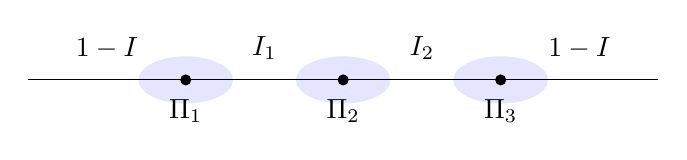
\begin{tikzpicture}

        \fill[blue!20, opacity=0.5] (2, 0) ellipse (0.6 and 0.3);
        \fill (2,0) circle (2pt);
        \node at (2, -0.4) {$\Pi_1$};

        \fill[blue!20, opacity=0.5] (4, 0) ellipse (0.6 and 0.3);
        \fill (4,0) circle (2pt);
        \node at (4, -0.4) {$\Pi_2$};

        \fill[blue!20, opacity=0.5] (6, 0) ellipse (0.6 and 0.3);
        \fill (6,0) circle (2pt);
        \node at (6, -0.4) {$\Pi_3$};

        \node at (1,0.4) {$1 - I$};
        \node at (3,0.4) {$I_1$};
        \node at (5,0.4) {$I_2$};
        \node at (7,0.4) {$1-I$};

        \draw (0,0) -- (8,0);
        
    \end{tikzpicture}
    \caption{\label{fig:interval shcematic} A schematic depiction}
\end{figure}
As was done in \cite{shap2017} we claim that:
\begin{equation}
    det(M)\approx det_{\Pi_1}(M) det_{\Pi_2}(M) det_{\Pi_3}(M)
\end{equation}
where $det_{\Pi_i}(M)$ is the determinant of $M$ restricted to the sites in $\Pi_i$.
Far from the intersection of $I_1, I_2$ we have $(1-I)\tilde P(1-I) + I\tilde PI = (1-I)P(1-I) + IPI$ therefore:
\begin{equation}
    \begin{split}
        &det_{\Pi_1}(M) det_{\Pi_3}(M) = \\
        &= det(1-P+P \left( (1-I)P(1-I) + IPI \right) P) \\
        &= Tr(\rho_I^2)\in\mathbb{R}_{>0}
    \end{split}
\end{equation}
Thus we are left with:
\begin{equation}
    arg(Z_{\mathcal{T}}) = arg(det(M)) = arg(det_{\Pi_2}(M))
\end{equation}
Using the quasidiagonality of $P$, we can continuously expand $I_1$ and $I_2$ without changing $det_{\Pi_2}(M)$ and therefore we can do the calculation in the limit of $I\rightarrow1$ and be left with:
\begin{equation}
    \lim_{I\rightarrow1}M=M_0=1-P+P\tilde PP=1-P(1-\tilde P)P
\end{equation}
In Appendix \ref{app:p_gamma_p} it is shown that $M_0$ is invertible, therefore, we can

write it's determinant as:
\begin{equation}
\label{eq:13}
    \begin{split}
        det(M_0)=exp\left(Tr\left(log\left(1-P(1-\tilde P)P\right)\right)\right)= \\
        =exp\left(-Tr\left(\sum_{n=1}^\infty\frac{\left(P(1-\tilde P)P\right)^n}{n}\right)\right)= \\
        =exp\left(-Tr\left(\sum_{n=1}^\infty\frac{1}{n\cdot2^n}\sum_{k=0}^n \begin{pmatrix}n \\ k\end{pmatrix}(-iP\tilde\Gamma P)^k\right)\right)
    \end{split}
\end{equation}
In Appendix \ref{app:p_gamma_p} we also prove that:
\begin{equation}
\label{eq:14}
    Im(Tr((-iP\tilde\Gamma P)^k)) = \left\{\begin{matrix} (-1)^m\nu(\Gamma) & k=2m+1 \\ 0 & k=2m\end{matrix}\right.
\end{equation}
If we substitute equation (\ref{eq:14}) into equation (\ref{eq:13}) we get:
\begin{equation}
    \begin{split}
        arg(Z_{\mathcal{T}}) &= -\sum_{n=1}^\infty\frac{1}{n\cdot2^n}\sum_{k=0}^{\left\lfloor\frac{n-1}{2}\right\rfloor} \begin{pmatrix}n \\ 2k+1\end{pmatrix}(-1)^k\nu(\Gamma)=\\
        &=-\nu(\Gamma)\sum_{n=1}^\infty\frac{1}{n}Im\left(\left(\frac{1+i}{2}\right)^n\right)=\\
        &=-\nu(\Gamma)Im\left(\sum_{n=1}^\infty\frac{1}{n}\left(\frac{1+i}{2}\right)^n\right)=\\
        &=-\nu(\Gamma)Im\left(log\left(1 - \frac{1+i}{2}\right)\right)=\frac{\pi}{4}\nu(\Gamma)
    \end{split}
\end{equation}

\begin{acknowledgments}
Thanks for everyone
\end{acknowledgments}

\appendix

\section{Properties of $P\tilde\Gamma P$}
\label{app:p_gamma_p}

In this section it will be useful to split $\Gamma$ into the diagonal and off diagonal matrices. We denote:
\begin{align}
    \Gamma=\Gamma_D + \Gamma_O \\
    \Gamma_D=\begin{pmatrix}\Gamma_{--} & 0 \\ 0 & \Gamma_{++} \end{pmatrix}, \;
    \Gamma_O=\begin{pmatrix}0 & \Gamma_{-+} \\ \Gamma_{+-} & 0 \end{pmatrix} \\
    \tilde\Gamma = T\Gamma T=\Gamma_D + i\tilde\Gamma_O
\end{align}
Using $\Gamma^2=-1$ it is straight forword to show the following relations:
\begin{align}
    \Gamma_D^2 + \Gamma_O^2 = -1, \; \{\Gamma_D,\Gamma_O\}=0 \label{eq:a4} \\
    [\Gamma_D,\tilde\Gamma_O]=[\Gamma_O,\tilde\Gamma_O]=0, \; \tilde\Gamma_O^2=\Gamma_O^2 \label{eq:a5}
\end{align}
The matrices $\Gamma_D,\Gamma_O$ and $\tilde\Gamma_O$ are real and skew symmetric, therefore, they are diagonalizable with purely imaginary eigenvalues. It follows that $[P,\tilde\Gamma_O]=0$ and therefore $P\tilde\Gamma_OP$ is also diagonalizable. In addition, $[P\tilde\Gamma_OP, P\Gamma_DP]=0$, and $iP\Gamma_DP$ is Hermitian, therefore $P\tilde\Gamma P$ is diagonalizable.\\
We will now show that the eigenvalues of $iP\tilde\Gamma P$ come in complex conjugate pairs unless they are $\pm i$. Since $\Gamma_O$ and $\tilde\Gamma_O$ commute, they have a common basis, let $v$ be an eigenvector in this basis:
\begin{align}
    \tilde\Gamma_Ov=i\lambda v, \; \Gamma_Ov=i\mu v \; (\mu=\pm\lambda)
\end{align}
Let us denote $u=\Gamma_Dv$ and from the commutation relations (\ref{eq:a4}), (\ref{eq:a5}) we have:
\begin{align}
    \tilde\Gamma_Ou=\tilde\Gamma_O\Gamma_Dv=\Gamma_D\tilde\Gamma_Ov=i\lambda\Gamma_Dv=i\lambda u \\
    \Gamma_Ou=\Gamma_O\Gamma_Dv=-\Gamma_D\Gamma_Ov=-i\mu\Gamma_Dv=-i\mu u \\
    \Gamma_Du=\Gamma_D^2v=(-1-\tilde\Gamma_O^2)v=(\lambda^2 - 1)v
\end{align}
If $|\lambda|<1$ then $u\ne0$, and we get a unique pairing between $v$ and $u$. In the subspace spanned by $v,\bar v,u,\bar u$ the eigenvectors of $iP\tilde\Gamma P$ are:
\begin{align}
    w_1=i(\mu+1)v + u, & w_2=i(-\mu+1)\bar v + \bar u \\
    w_3=i(\mu-1)v + u, & w_4=i(-\mu-1)\bar v + \bar u
\end{align}
The first two eigenvectors are with eigenvalues $\alpha_\pm=\lambda^2-1 \pm i\lambda$ and the second two with $0$. However, if $\lambda=\pm1$ then $u=0$ and $\mu=\pm1$ so one of $w_1, w_2$ is zero.\\
Using the structure of the eigenvalues we can see that for $|\lambda|<1, Im(\alpha_+^k+\alpha_-^k)=0$ therefore:
\begin{equation}
\label{eq:a12}
    \begin{split}
        &Im\left(Tr\left((-iP\tilde\Gamma P)^k\right)\right)=\sum_{j}Im\left(\alpha_j^k\right)= \\
        &=\sum_{j,\lambda_j=\pm1}Im\left(\alpha_j^k\right)= \\
        &=\left\{\begin{matrix} (-1)^mIm\left(Tr(-iP\tilde\Gamma P)\right) & k=2m+1 \\ 0 & k=2m\end{matrix}\right.
    \end{split}
\end{equation}
Since $\Gamma$ and $\tilde\Gamma$ are parity flipping, the trace of an odd product of them is zero. Using this we can simplify (\ref{eq:a12}) and prove (\ref{eq:14}):
\begin{equation}
    \begin{split}
        Im(Tr(-iP\tilde\Gamma P)) = -\frac{Im(Tr(\{\Gamma,\tilde\Gamma\}))}{4} = \nu(\Gamma) \\
        Im(Tr((-iP\tilde\Gamma P)^k)) = \left\{\begin{matrix} (-1)^m\nu(\Gamma) & k=2m+1 \\ 0 & k=2m\end{matrix}\right.
    \end{split}
\end{equation}
This derivation can also be utilized to show that $M_0=1-P+P\tilde PP$ is invertible. For any eigenvector $v$ of $M_0$ that is in the subspace of $P$ ($Pv=v$), we have $M_0v=\frac{(1-(\lambda^2-1\pm i\lambda))}{2}v$, which is never 0 for any real $|\lambda|\le1$. $M_0$ acts as the identity on the complementary subspace, therefore $det(M_0)\ne0$.

\nocite{*}

\bibliography{apssamp}% Produces the bibliography via BibTeX.

\end{document}
%
% ****** End of file apssamp.tex ******
